\pagestyle{empty}

\section*{The Setting}
We work in a compact, riemanian, orientable, smooth Manifold $(M,g)$ of dimension $m$ together with a Morse-Smale funktion 
\begin{align}
    f: M\to \R
\end{align}
We assume that $q$ is a critical point of index $k+1$ and $p$ is a critical point of index $k$. we define $f(q)=b$ and $f(p)=a$ and assume that there is no kritical point in $f^{-1}(a,b)\subseteq M$. We define the sub and superlevelsets 
\begin{align}
    M^t:=\{ x\in M | f(x)\leq t \} \quad \text{and}\quad M_t:=\{ x\in M | f(x)\geq t \} \, ,
\end{align} and the constants 
\begin{align}
    c \in (a,b) \quad , \quad \epsilon >0 \text{ small } \quad,\quad T>0 \text{ big .}
\end{align} With this we define the sets: 
\begin{align}
	N_q  & \coloneq    \{ x\in M_c |f(\phi_{-T}(x))  \leq b+ \epsilon  \}   \, ,  \\
	L_q  & \coloneq    \{ x\in N_q |f(x)             =    c            \}    \, , \\
	N_p  & \coloneq    \{ x\in M^c |f(\phi_T(x))     \geq a-\epsilon   \}    \, , \\
	L_p  & \coloneq    \{ x\in N_p |f( \phi_T(x))    =    a-\epsilon   \} \, ,
\end{align} and finally: 
\begin{align}
	C  & \coloneq  N_p \cup N_q  \, ,                     \\
	B  & \coloneq  N_p \cup L_q   \, ,                   \\
	A  & \coloneq  L_p \cup \mathring{(L_q-N_p)} \, .
\end{align}
\begin{lemma}\label{lem: The Main Lemma Np is tubular}
    We claim that 
    \begin{enumerate}
	\item $(N_q,L_q)$ is a regular index pair for $q$\, . \label{lem: enum: 1}
	\item $(C,B)$ is an index pair for $q$\, .\label{lem: enum: 2}
	\item $(N_p,L_p)$ is a regular index pair for $p$\, .\label{lem: enum: 3}
	\item $(B,A)$ is an index pair for $p$\, .\label{lem: enum: 4}
    \item $N_p$ is homotopically equivalent to a tubular neighbourhood of $W(\to p)\cap M^c$\, .\label{lem: enum: 5}
\end{enumerate}
\end{lemma}

    The statements \ref{lem: enum: 1}-\ref{lem: enum: 4} are easy to proof by the definitions. The regularity can be derived from a general fact for pairs $(X,Y)$ in metric spaces: If $Y$ is closed in $X$ and there is a neighbourhood of $Y$ that is open in $X$ such that $Y$ is a strong deformation retract of $U$. So the only thing left to show is, that $N_p$ is a tubular neighbourhood. in \cite{MorseTheorySalmbon} in the proof of lemma 3.2 Salamon claims this to be true without a proof (page 119 in the attached source). Similar, in \cite{banyaga2004lectures} Banyaga claims this (also without any argument).
  I find this difficult to proof, since we cannot use the flow for the map from the normal bundle, as points leave $N_p$ along the flow: The Set $N_p$ is sketched in the figure below. 
    \begin{center}
        

\tikzset{every picture/.style={line width=0.75pt}} %set default line width to 0.75pt        
\resizebox{\linewidth}{!}{%



\tikzset{every picture/.style={line width=0.75pt}} %set default line width to 0.75pt      

\tikzset{every picture/.style={line width=0.75pt}} %set default line width to 0.75pt        

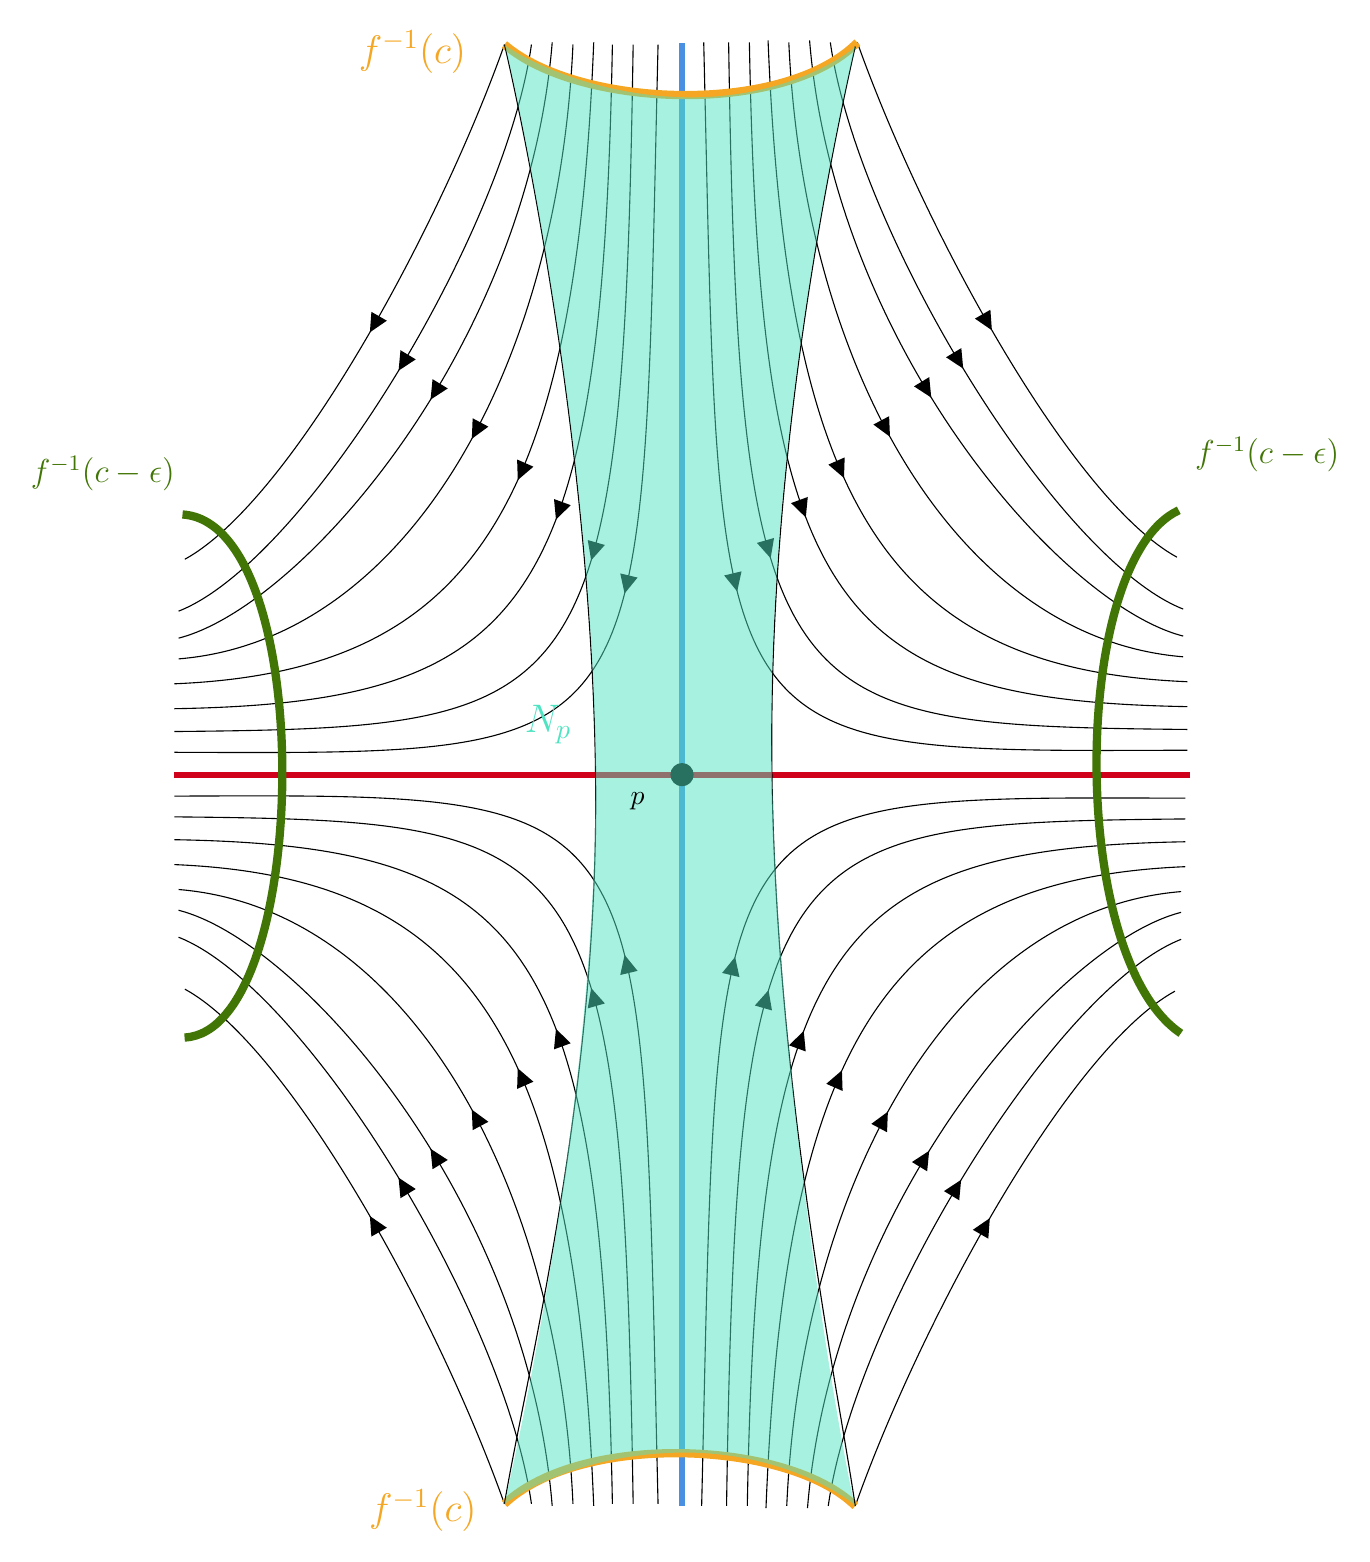
\begin{tikzpicture}[x=0.75pt,y=0.75pt,yscale=-1,xscale=1]
%uncomment if require: \path (0,843); %set diagram left start at 0, and has height of 843

%Straight Lines [id:da11875089429305197] 
\draw [color={rgb, 255:red, 74; green, 144; blue, 226 }  ,draw opacity=1 ][line width=2.25]    (329,31.6) -- (329,736.43) ;
%Straight Lines [id:da5325201497809933] 
\draw [color={rgb, 255:red, 208; green, 2; blue, 27 }  ,draw opacity=1 ][line width=2.25]    (84.42,384.02) -- (573.58,384.02) ;
%Shape: Circle [id:dp07579894054308489] 
\draw  [draw opacity=0][fill={rgb, 255:red, 0; green, 0; blue, 0 }  ,fill opacity=1 ] (323.4,384.02) .. controls (323.4,380.92) and (325.91,378.42) .. (329,378.42) .. controls (332.09,378.42) and (334.6,380.92) .. (334.6,384.02) .. controls (334.6,387.11) and (332.09,389.62) .. (329,389.62) .. controls (325.91,389.62) and (323.4,387.11) .. (323.4,384.02) -- cycle ;
%Curve Lines [id:da1665503577346341] 
\draw    (339.45,31.25) .. controls (347.8,378.2) and (336.45,373.05) .. (572.45,372.25) ;
\draw [shift={(355.57,295.75)}, rotate = 256.55] [fill={rgb, 255:red, 0; green, 0; blue, 0 }  ][line width=0.08]  [draw opacity=0] (8.93,-4.29) -- (0,0) -- (8.93,4.29) -- cycle    ;
%Curve Lines [id:da7994448259938868] 
\draw    (351.45,31.25) .. controls (356.45,355.25) and (373.45,360.25) .. (572.45,362.25) ;
\draw [shift={(371.68,279.76)}, rotate = 253.92] [fill={rgb, 255:red, 0; green, 0; blue, 0 }  ][line width=0.08]  [draw opacity=0] (8.93,-4.29) -- (0,0) -- (8.93,4.29) -- cycle    ;
%Curve Lines [id:da558792425961241] 
\draw    (361.45,31.25) .. controls (366.45,302.25) and (401.45,348.25) .. (572.45,351.25) ;
\draw [shift={(388.63,260.1)}, rotate = 249.87] [fill={rgb, 255:red, 0; green, 0; blue, 0 }  ][line width=0.08]  [draw opacity=0] (8.93,-4.29) -- (0,0) -- (8.93,4.29) -- cycle    ;
%Curve Lines [id:da5211576581151481] 
\draw    (370.45,30.25) .. controls (379.45,254.25) and (428.45,333.25) .. (572.45,339.25) ;
\draw [shift={(407.03,241.09)}, rotate = 246.23] [fill={rgb, 255:red, 0; green, 0; blue, 0 }  ][line width=0.08]  [draw opacity=0] (8.93,-4.29) -- (0,0) -- (8.93,4.29) -- cycle    ;
%Curve Lines [id:da39021575553782684] 
\draw    (380.45,31.25) .. controls (387.45,187.25) and (460.45,318.25) .. (570.45,327.25) ;
\draw [shift={(429.18,221.22)}, rotate = 242] [fill={rgb, 255:red, 0; green, 0; blue, 0 }  ][line width=0.08]  [draw opacity=0] (8.93,-4.29) -- (0,0) -- (8.93,4.29) -- cycle    ;
%Curve Lines [id:da6126506516051217] 
\draw    (390.45,30.25) .. controls (402.45,177.25) and (511.45,302.25) .. (570.45,317.25) ;
\draw [shift={(449.07,202.35)}, rotate = 238.74] [fill={rgb, 255:red, 0; green, 0; blue, 0 }  ][line width=0.08]  [draw opacity=0] (8.93,-4.29) -- (0,0) -- (8.93,4.29) -- cycle    ;
%Curve Lines [id:da24082042581971141] 
\draw    (400.45,31.25) .. controls (413.45,123.25) and (509.45,280.25) .. (570.45,304.25) ;
\draw [shift={(464.47,188.39)}, rotate = 239.04] [fill={rgb, 255:red, 0; green, 0; blue, 0 }  ][line width=0.08]  [draw opacity=0] (8.93,-4.29) -- (0,0) -- (8.93,4.29) -- cycle    ;
%Curve Lines [id:da5298362087143788] 
\draw    (413.45,31.25) .. controls (445.45,121.25) and (516.45,251.25) .. (567.45,279.25) ;
\draw [shift={(478.29,169.92)}, rotate = 240.15] [fill={rgb, 255:red, 0; green, 0; blue, 0 }  ][line width=0.08]  [draw opacity=0] (8.93,-4.29) -- (0,0) -- (8.93,4.29) -- cycle    ;

%Curve Lines [id:da21918221686589523] 
\draw    (317.45,32.25) .. controls (309.1,379.2) and (320.45,374.05) .. (84.45,373.25) ;
\draw [shift={(301.33,296.75)}, rotate = 283.45] [fill={rgb, 255:red, 0; green, 0; blue, 0 }  ][line width=0.08]  [draw opacity=0] (8.93,-4.29) -- (0,0) -- (8.93,4.29) -- cycle    ;
%Curve Lines [id:da34745008178206616] 
\draw    (305.45,32.25) .. controls (300.45,356.25) and (283.45,361.25) .. (84.45,363.25) ;
\draw [shift={(285.22,280.76)}, rotate = 286.08] [fill={rgb, 255:red, 0; green, 0; blue, 0 }  ][line width=0.08]  [draw opacity=0] (8.93,-4.29) -- (0,0) -- (8.93,4.29) -- cycle    ;
%Curve Lines [id:da8640093846313118] 
\draw    (295.45,32.25) .. controls (290.45,303.25) and (255.45,349.25) .. (84.45,352.25) ;
\draw [shift={(268.27,261.1)}, rotate = 290.13] [fill={rgb, 255:red, 0; green, 0; blue, 0 }  ][line width=0.08]  [draw opacity=0] (8.93,-4.29) -- (0,0) -- (8.93,4.29) -- cycle    ;
%Curve Lines [id:da925990106139973] 
\draw    (286.45,31.25) .. controls (277.45,255.25) and (228.45,334.25) .. (84.45,340.25) ;
\draw [shift={(249.87,242.09)}, rotate = 293.77] [fill={rgb, 255:red, 0; green, 0; blue, 0 }  ][line width=0.08]  [draw opacity=0] (8.93,-4.29) -- (0,0) -- (8.93,4.29) -- cycle    ;
%Curve Lines [id:da08743123557319321] 
\draw    (276.45,32.25) .. controls (269.45,188.25) and (196.45,319.25) .. (86.45,328.25) ;
\draw [shift={(227.72,222.22)}, rotate = 298] [fill={rgb, 255:red, 0; green, 0; blue, 0 }  ][line width=0.08]  [draw opacity=0] (8.93,-4.29) -- (0,0) -- (8.93,4.29) -- cycle    ;
%Curve Lines [id:da08430775562121551] 
\draw    (266.45,31.25) .. controls (254.45,178.25) and (145.45,303.25) .. (86.45,318.25) ;
\draw [shift={(207.83,203.35)}, rotate = 301.26] [fill={rgb, 255:red, 0; green, 0; blue, 0 }  ][line width=0.08]  [draw opacity=0] (8.93,-4.29) -- (0,0) -- (8.93,4.29) -- cycle    ;
%Curve Lines [id:da38820398572752524] 
\draw    (256.45,32.25) .. controls (243.45,124.25) and (147.45,281.25) .. (86.45,305.25) ;
\draw [shift={(192.43,189.39)}, rotate = 300.96] [fill={rgb, 255:red, 0; green, 0; blue, 0 }  ][line width=0.08]  [draw opacity=0] (8.93,-4.29) -- (0,0) -- (8.93,4.29) -- cycle    ;
%Curve Lines [id:da5677669307058717] 
\draw    (243.45,32.25) .. controls (211.45,122.25) and (140.45,252.25) .. (89.45,280.25) ;
\draw [shift={(178.61,170.92)}, rotate = 299.85] [fill={rgb, 255:red, 0; green, 0; blue, 0 }  ][line width=0.08]  [draw opacity=0] (8.93,-4.29) -- (0,0) -- (8.93,4.29) -- cycle    ;

%Curve Lines [id:da5375642083324416] 
\draw    (338.45,736.36) .. controls (346.8,389.41) and (335.45,394.56) .. (571.45,395.36) ;
\draw [shift={(354.57,471.87)}, rotate = 103.45] [fill={rgb, 255:red, 0; green, 0; blue, 0 }  ][line width=0.08]  [draw opacity=0] (8.93,-4.29) -- (0,0) -- (8.93,4.29) -- cycle    ;
%Curve Lines [id:da5126738644229648] 
\draw    (350.45,736.36) .. controls (355.45,412.36) and (372.45,407.36) .. (571.45,405.36) ;
\draw [shift={(370.68,487.86)}, rotate = 106.08] [fill={rgb, 255:red, 0; green, 0; blue, 0 }  ][line width=0.08]  [draw opacity=0] (8.93,-4.29) -- (0,0) -- (8.93,4.29) -- cycle    ;
%Curve Lines [id:da5839119584885231] 
\draw    (360.45,736.36) .. controls (365.45,465.36) and (400.45,419.36) .. (571.45,416.36) ;
\draw [shift={(387.63,507.52)}, rotate = 110.13] [fill={rgb, 255:red, 0; green, 0; blue, 0 }  ][line width=0.08]  [draw opacity=0] (8.93,-4.29) -- (0,0) -- (8.93,4.29) -- cycle    ;
%Curve Lines [id:da975815253328843] 
\draw    (369.45,737.36) .. controls (378.45,513.36) and (427.45,434.36) .. (571.45,428.36) ;
\draw [shift={(406.03,526.52)}, rotate = 113.77] [fill={rgb, 255:red, 0; green, 0; blue, 0 }  ][line width=0.08]  [draw opacity=0] (8.93,-4.29) -- (0,0) -- (8.93,4.29) -- cycle    ;
%Curve Lines [id:da9314613290760876] 
\draw    (379.45,736.36) .. controls (386.45,580.36) and (459.45,449.36) .. (569.45,440.36) ;
\draw [shift={(428.18,546.4)}, rotate = 118] [fill={rgb, 255:red, 0; green, 0; blue, 0 }  ][line width=0.08]  [draw opacity=0] (8.93,-4.29) -- (0,0) -- (8.93,4.29) -- cycle    ;
%Curve Lines [id:da09174306781681929] 
\draw    (389.45,737.36) .. controls (401.45,590.36) and (510.45,465.36) .. (569.45,450.36) ;
\draw [shift={(448.07,565.26)}, rotate = 121.26] [fill={rgb, 255:red, 0; green, 0; blue, 0 }  ][line width=0.08]  [draw opacity=0] (8.93,-4.29) -- (0,0) -- (8.93,4.29) -- cycle    ;
%Curve Lines [id:da21494064860512774] 
\draw    (399.45,736.36) .. controls (412.45,644.36) and (508.45,487.36) .. (569.45,463.36) ;
\draw [shift={(463.47,579.22)}, rotate = 120.96] [fill={rgb, 255:red, 0; green, 0; blue, 0 }  ][line width=0.08]  [draw opacity=0] (8.93,-4.29) -- (0,0) -- (8.93,4.29) -- cycle    ;
%Curve Lines [id:da506519829239\end{proo7652] 
\draw    (412.45,736.36) .. controls (444.45,646.36) and (515.45,516.36) .. (566.45,488.36) ;
\draw [shift={(477.29,597.7)}, rotate = 119.85] [fill={rgb, 255:red, 0; green, 0; blue, 0 }  ][line width=0.08]  [draw opacity=0] (8.93,-4.29) -- (0,0) -- (8.93,4.29) -- cycle    ;

%Curve Lines [id:da3880154567702636] 
\draw    (317.45,735.36) .. controls (309.1,388.41) and (320.45,393.56) .. (84.45,394.36) ;
\draw [shift={(301.33,470.87)}, rotate = 76.55] [fill={rgb, 255:red, 0; green, 0; blue, 0 }  ][line width=0.08]  [draw opacity=0] (8.93,-4.29) -- (0,0) -- (8.93,4.29) -- cycle    ;
%Curve Lines [id:da9327211409936709] 
\draw    (305.45,735.36) .. controls (300.45,411.36) and (283.45,406.36) .. (84.45,404.36) ;
\draw [shift={(285.22,486.86)}, rotate = 73.92] [fill={rgb, 255:red, 0; green, 0; blue, 0 }  ][line width=0.08]  [draw opacity=0] (8.93,-4.29) -- (0,0) -- (8.93,4.29) -- cycle    ;
%Curve Lines [id:da09647590503157577] 
\draw    (295.45,735.36) .. controls (290.45,464.36) and (255.45,418.36) .. (84.45,415.36) ;
\draw [shift={(268.27,506.52)}, rotate = 69.87] [fill={rgb, 255:red, 0; green, 0; blue, 0 }  ][line width=0.08]  [draw opacity=0] (8.93,-4.29) -- (0,0) -- (8.93,4.29) -- cycle    ;
%Curve Lines [id:da15668737739736305] 
\draw    (286.45,736.36) .. controls (277.45,512.36) and (228.45,433.36) .. (84.45,427.36) ;
\draw [shift={(249.87,525.52)}, rotate = 66.23] [fill={rgb, 255:red, 0; green, 0; blue, 0 }  ][line width=0.08]  [draw opacity=0] (8.93,-4.29) -- (0,0) -- (8.93,4.29) -- cycle    ;
%Curve Lines [id:da5883237308999977] 
\draw    (276.45,735.36) .. controls (269.45,579.36) and (196.45,448.36) .. (86.45,439.36) ;
\draw [shift={(227.72,545.4)}, rotate = 62] [fill={rgb, 255:red, 0; green, 0; blue, 0 }  ][line width=0.08]  [draw opacity=0] (8.93,-4.29) -- (0,0) -- (8.93,4.29) -- cycle    ;
%Curve Lines [id:da9204033290837756] 
\draw    (266.45,736.36) .. controls (254.45,589.36) and (145.45,464.36) .. (86.45,449.36) ;
\draw [shift={(207.83,564.26)}, rotate = 58.74] [fill={rgb, 255:red, 0; green, 0; blue, 0 }  ][line width=0.08]  [draw opacity=0] (8.93,-4.29) -- (0,0) -- (8.93,4.29) -- cycle    ;
%Curve Lines [id:da49739155745577546] 
\draw    (256.45,735.36) .. controls (243.45,643.36) and (147.45,486.36) .. (86.45,462.36) ;
\draw [shift={(192.43,578.22)}, rotate = 59.04] [fill={rgb, 255:red, 0; green, 0; blue, 0 }  ][line width=0.08]  [draw opacity=0] (8.93,-4.29) -- (0,0) -- (8.93,4.29) -- cycle    ;
%Curve Lines [id:da32213499249738287] 
\draw    (243.45,735.36) .. controls (211.45,645.36) and (140.45,515.36) .. (89.45,487.36) ;
\draw [shift={(178.61,596.7)}, rotate = 60.15] [fill={rgb, 255:red, 0; green, 0; blue, 0 }  ][line width=0.08]  [draw opacity=0] (8.93,-4.29) -- (0,0) -- (8.93,4.29) -- cycle    ;


%Curve Lines [id:da05541171078629925] 
\draw [color={rgb, 255:red, 245; green, 166; blue, 35 }  ,draw opacity=1 ][line width=3]    (243.45,32.25) .. controls (279.42,63.08) and (378.33,66.67) .. (413.45,31.25) ;
%Curve Lines [id:da4989004892868002] 
\draw [color={rgb, 255:red, 245; green, 166; blue, 35 }  ,draw opacity=1 ][line width=3]    (243.45,735.36) .. controls (280.33,700.67) and (380.33,704.67) .. (412.45,736.36) ;
%Curve Lines [id:da44411839842500755] 
\draw [color={rgb, 255:red, 65; green, 117; blue, 5 }  ,draw opacity=1 ][line width=3]    (88.33,258.67) .. controls (154.22,262.97) and (150.33,507.67) .. (89.33,510.67) ;
%Curve Lines [id:da05367202270104565] 
\draw [color={rgb, 255:red, 65; green, 117; blue, 5 }  ,draw opacity=1 ][line width=3]    (568.33,256.67) .. controls (516.33,280.67) and (514.33,471.67) .. (569.33,508.67) ;
%Curve Lines [id:da7969530986481941] 
\draw    (243.45,32.25) .. controls (254.33,78.67) and (285.1,230.49) .. (287.33,382.67) .. controls (289.57,534.85) and (253.34,675.31) .. (243.45,735.36) ;
%Curve Lines [id:da5283140439270424] 
\draw    (412.45,33.25) .. controls (400.33,86.67) and (370.1,232.49) .. (372.33,384.67) .. controls (374.57,536.85) and (404.33,680.67) .. (412.45,736.36) ;

%Shape: Polygon Curved [id:ds3817941045439226] 
\draw  [draw opacity=0][fill={rgb, 255:red, 80; green, 227; blue, 194 }  ,fill opacity=0.5 ] (243.45,735.36) .. controls (243.39,735.01) and (288.33,547.67) .. (287.33,382.67) .. controls (286.33,217.67) and (244.39,31.96) .. (243.45,32.25) .. controls (242.51,32.54) and (278.33,56.67) .. (330.33,57.67) .. controls (382.33,58.67) and (412.39,33.99) .. (412.45,33.25) .. controls (412.51,32.51) and (368.33,212.67) .. (372.33,384.67) .. controls (376.33,556.67) and (411.01,736.21) .. (412.45,736.36) .. controls (413.89,736.52) and (381.33,709.67) .. (327.33,710.67) .. controls (273.33,711.67) and (243.51,735.72) .. (243.45,735.36) -- cycle ;

% Text Node
\draw (303,391.4) node [anchor=north west][inner sep=0.75pt]    {$p$};
% Text Node
\draw (172,24.4) node [anchor=north west][inner sep=0.75pt]  [font=\Large,color={rgb, 255:red, 245; green, 166; blue, 35 }  ,opacity=1 ]  {$f^{-1}( c)$};
% Text Node
\draw (177,727.07) node [anchor=north west][inner sep=0.75pt]  [font=\Large,color={rgb, 255:red, 245; green, 166; blue, 35 }  ,opacity=1 ]  {$f^{-1}( c)$};
% Text Node
\draw (14,229.4) node [anchor=north west][inner sep=0.75pt]  [font=\large,color={rgb, 255:red, 65; green, 117; blue, 5 }  ,opacity=1 ]  {$f^{-1}( c-\epsilon )$};
% Text Node
\draw (575,220.4) node [anchor=north west][inner sep=0.75pt]  [font=\large,color={rgb, 255:red, 65; green, 117; blue, 5 }  ,opacity=1 ]  {$f^{-1}( c-\epsilon )$};
% Text Node
\draw (252,349.4) node [anchor=north west][inner sep=0.75pt]  [font=\Large,color={rgb, 255:red, 80; green, 227; blue, 194 }  ,opacity=1 ]  {$N_{p}$};


\end{tikzpicture}


}
    \end{center}
So to proof this, we first formulate two lemmas. First we restate/ refine the $\lambda$-lemma: 
\begin{lemma}[The Technical $\lambda-$Lemma] 
	Let $ M$ \todo{parameter dependence einfügen}be a smooth manifold and let $p$ be a hyperbolic fixpoint of a diffeomorphism $\phi$ on $M$ with $\dim W(p \to)=r$ for ${0<r<m=\dim M}$. Let $N$ be an injective immersed submanifold of $M$ that is invariant under $\phi$ and has a point of transverse intersection $q$ with $W(\to p)$. Then for any $\epsilon>0$, any $r-$cell neighbourhood $D$ of $q$ in $N$ that also intersects $W(\to p)$ transversal and any $r-cell$ neighbourhood $B$ of $p$ in $W(p\to))$ there is a smaller cell $\tilde{D}\subset D$, an $n\in \N$ such that the following is true:
	
	We can assume that $B$ and $\phi^n(\tilde{D})$ lives in a chart centered at $p$ with a product structure $U\cong W(\to p)\cap B_\mu(0)\times W(p\to)\cap B_\mu(0)$. Here,the invers of the projection into $B\subseteq W(\to p)$:
	\begin{equation*}
		h: B\to \phi^n(\tilde{D})\, 
	\end{equation*}satisfies:
	\begin{enumerate}
		\item $\sup_{x \in B}\norm{x-h(x)}<\epsilon$ and
		\item For the inclusions  $i_1:B\to M$ and $i_2:\phi^n(\tilde{D})\to M$ we have that 
		\begin{equation*}
			\sup_{x \in B}\norm{\diff(i_1)_x-\diff(i_2\circ h)_x}<\epsilon\, .
		\end{equation*}
	\end{enumerate}
\end{lemma}
	\begin{proof}
		Let \( q \) be a point of transversal intersection of \( W(\to p) \) with \( N \). Since both \( N \) and \( W(\to p) \) are invariant under \( \phi \), it follows that \( \phi^n(q) \in N \cap W(\to p) \) for all \( n \in \N \). Moreover, the intersection remains transversal: the direct sum decomposition \( T_q M = T_q W(\to p) \oplus T_q N \) is preserved under \( d\phi_q \), which implies transversality at \( \phi^n(q) \) as well.
		
		Therefore, we may assume that \( q \) lies in a coordinate chart centered at the hyperbolic fixed point \( p \), and identify a neighborhood of \( p \) with an open subset of \( \mathbb{R}^m \), where \( m = \dim M \). By hyperbolicity of \( p \), the tangent space at \( p \) splits as
		\[
		T_p M = T^s_p M \oplus T^u_p M,
		\]
		and this splitting is preserved by \( d\phi_p \). As discussed earlier\todo{reference einfügen}, there exists a chart in which \( d\phi_p \) is represented by a real diagonal matrix (in suitable coordinates)\todo{in fact we can choose a Morse chart that satisfies this!}. Hence, we may choose an orthonormal basis of coordinates \( (x_s, x_u) \in \mathbb{R}^s \times \mathbb{R}^u \), adapted to the stable and unstable subspaces, such that
		\[
		d\phi_0 =
		\begin{pmatrix}
			A & 0 \\
			0 & B
		\end{pmatrix},
		\]
		where the eigenvalues of \( A \) have modulus less than 1, and those of \( B \) greater than 1.
		
		Since we are working in \( \mathbb{R}^m \), we identify the manifold and its tangent space locally around 0. We then expand \( \phi \) in a Taylor series at the origin:
		\[
		\phi(x_s, x_u) = \phi(0) + d\phi_0(x_s, x_u) + f(x_s, x_u),
		\]
		where \( f(0) = 0 \) and \( df(0) = 0 \). Writing this in coordinates gives:
		\begin{equation} \label{eq: proof of Lambda lemma phi split}
			\phi(x_s, x_u) = (A x_s + f_s(x_s, x_u),\; B x_u + f_u(x_s, x_u)).
		\end{equation}
  Furthermore, since $f=\phi-\diff \phi|_0$ we know that: 
		\begin{align*}
			\frac{\partial f_s}{\partial x_u}|_{(0,x_u)}=\frac{\partial \phi_s}{\partial x_u}|_{(0,x_u)}=0=\frac{\partial f_u}{\partial x_s}|_{(x_s,0)}=\frac{\partial \phi_u}{\partial x_s}|_{(x_s,0)}.
		\end{align*} Similar to Corollary $\ref{cor: Tangendspace splits}$ we can define an inner product such that for the operator norm we have 
		\begin{align*}
			\norm{A}\leq \alpha <1 \quad \text{ and } \quad \norm{B^{-1}}\leq \frac{1}{\beta} <1.
		\end{align*}
		Since $1=\norm{\id}=\norm{BB^{-1}}\leq \norm{B}\cdot \norm{B^{-1}}$ we know that $\norm{B}\geq \beta$.
		For a neighbourhood $U_1\subseteq U$ of the origin we define 
		\begin{align*}
			k:=\max_{i,j=s,u} \Bigg\{ \sup_{\overline{U_1}}\norm{\frac{\partial f_i}{\partial x_j}} \Bigg\},
		\end{align*} and choose $U_1$ small enough such that $k$ satisfies:
		
		
		\begin{gather*}
			0<k<1 \\
			\beta_1:=\beta -k >1 \\
			\alpha_1:=\alpha +k <1 \\
			k<\frac{1}{4}(b_1-1)^2.
		\end{gather*}
		This can be achieved since $\diff f\big|_0=0$.
		Let $B$ be a cell neighbourhood of the origin in $W(p\to )$. For some $n \in \N$ we have that $\phi^{-n}(B)\subseteq U_1$. If the $\lambda-$lemma holds for $\phi^{-n}(B)$ for all $\epsilon$ it also holds for $B$, since the metric and $\phi$ are continuous and the $r-$cell is compact. Therefore, the change of distance after applying $\phi^{-n}$ is finite and we can choose the distance from $\phi^{-n}(B)$ to $D$ small enough such that $B$ is $\epsilon~C^1$-close to $D$. Hence, without restrictions $B\subseteq U_1$ and $q\in U_1$.  Next we define the inclination of $N$ with respect to the (un-)stable manifolds as follows: 
		
		Let $x\subseteq N \cap U_1$ and $v^0\in T_xN\subseteq T_0M=T^s_0M \oplus T^u_oM$ and let $v^0=(v_s^0,v_u^0)$ be the coordinate entries. Furthermore let $v$ be a unit vector. Now we define the \textbf{inclination} of $v^0$:
		\begin{align*}
			\lambda(v^0)=\frac{\norm{v^0_s}}{\norm{v^0_u}}.
		\end{align*}
		In other words: The smaller the inclination, the more parallel we are to $W(p\to)$. Notive how we can only define the inclination if $v^0_u\neq 0$. 
		Furthermore define:
		\begin{align*} x^n:=\phi^n(x), ~v^n:= \diff \phi_{x^{n-1}}(v^{n-1}) \text{ and } \phi(x)=(\phi_s(x),\phi_u(x))\in W(\to 0)\times W(0\to).
		\end{align*}
		Now we want to calculate the derivative $\diff \phi|_{q^n}$. But first inspect:
		\begin{align*}
			\diff \phi|_x=\begin{pmatrix}
				\frac{\partial \phi_s}{\partial x_s}|_{x} & \frac{\partial \phi_s}{\partial x_u} |_{x}\\
				\frac{\partial \phi_u}{\partial x_s} |_{x}& \frac{\partial \phi_u}{\partial x_u}|_{x}
			\end{pmatrix}\overset{(\ref{eq: proof of Lambda lemma phi split}) }{~=~}
			\begin{pmatrix}
				A+ \frac{\partial f_s}{\partial x_s}|_{x}& \frac{\partial f_s}{\partial x_u}|_{x}\\
				\frac{\partial f_u}{\partial x_s} |_{x} & B+ \frac{\partial f_u}{\partial x_u}|_{x}
			\end{pmatrix} 
		\end{align*} Since $q^n\in W(\to 0)$ and $\frac{\partial f_u}{\partial x_s}(x_s,u)$=0 this gives us:
		
		\begin{align*}
			\diff \phi|_{q^n}=\begin{pmatrix}
				A+ \frac{\partial f_s}{\partial x_s}|_{q^n}&    \frac{\partial f_s}{\partial x_u}|_{q^n}\\
				0                                   & B+ \frac{\partial f_u}{\partial x_u}|_{q^n}
			\end{pmatrix} 
		\end{align*}
		Let $B_s(\delta)$ denote the ball of radius $\delta$ around the origin that lives in $W(\to p)$ and $U_2:= B_s(\delta)\times B$. Since $\frac{\partial f_s}{\partial x_u}|_{(0,x_u)}=0$ and by the smoothness of  $\phi$, for any $\epsilon >0$ there exists a $\delta$ such that 
		\begin{align*}
			\underbrace{\sup_{U_2}\norm{\frac{\partial f_s}{\partial x_u}}}_{:=k_1}< \min\{\epsilon, k \}.
		\end{align*} 
 Again, we assume $q\in D\subseteq  U_2$. Now we want to get a hold of the inclination:  Let $x\in N$ such that $x^j\in U_2 $ for all $j\leq n$ and let $v^0\in T_xN$. Denote $v^n=(v^n_s,v^n_u)\in T_0W(\to 0)\times T_0W(0 \to)$. 
		\begin{align}
			\lambda(v^n)&= \frac{\norm{\diff \phi_s|_{x^{n-1}}(v^{n-1})}}{\norm{\diff \phi_u|_{x^{n-1}}(v^{n-1})}} \nonumber \\
			&=\frac{\norm{Av_s^{n-1} +\ \frac{\partial f_s}{\partial x_s}|_{x^{n-1}}v_s^{n-1} \ \, + \, \frac{\partial f_s}{\partial x_u}|_{x^{n-1}}(v_u^{n-1})}}{\norm{\color{blue} \frac{\partial f_u}{\partial x_s}|_{x^{n-1}}(v_s^{n-1}) \color{black}+   Bv_u^{n-1}+\frac{\partial f_u}{\partial x_u}|_{x^{n-1}}(v_u^{n-1})}} \nonumber \\
			& \leq \frac{ (\alpha +k )\norm{v_s^{n-1}}+k_1 \norm{(v_u^{n-1})}}
			{ \color{blue}k \norm{(v_s^{n-1})} \color{black}  +  (\beta+k)\norm{ v_u^{n-1}}} \nonumber \\
			& \leq \frac{ (\alpha +k )\norm{v_s^{n-1}}+k_1 \norm{(v_u^{n-1})}}
			{ (\beta-k)\norm{ v_u^{n-1}}  - \color{blue} k_1 \norm{(v_s^{n-1})} \color{black} } &\quad \text{since } \beta-k>1 \text{ and }k_1<k<1 \nonumber \\
			& = \frac{ (\alpha +k )\lambda(v^{n-1})+k_1}
			{ \beta_1  - \color{blue} k_1 \lambda{v^{n-1}\color{black} }} &\quad \text{we divided by }\norm{v_u^{n-1}} \nonumber \\
			&\leq \frac{\lambda(v^{n-1})+k_1}
			{ \beta_1  - \color{blue} k_1 \lambda(v^{n-1}) \color{black} }  \label{eq: estimate lambda(v^n)}				
		\end{align} 
		If $x\in W(\to 0)$ the blue part above disappears and we get:
		\begin{align*}
			\lambda(v^n) \leq \frac{\lambda(v^{n-1})+k_1}{\beta_1}.
		\end{align*} By induction we get:
		\begin{align}
			\lambda(v^n)\leq \frac{\lambda(v^{n-1})+k_1}{\beta_1}=\frac{\frac{\lambda(v^{n-2})+k_1}{\beta_1}+k_1}{\beta_1}= \frac{\frac{\lambda(v^{n-2})+\frac{k_1 \beta_1}{\beta_1}}{\beta_1}+k_1}{\beta_1} =\frac{\lambda(v^{n-2})+k_1+ k_1 \beta_1}{\beta_1^2}\leq \cdots \nonumber \\
			\leq \frac{\lambda(v^0)+\sum_{l=0}^{n-1}k_1 \beta_1^l}{\beta_1^n}~. \label{eq: proof lambda lemma estimate lambda(v^n) with x=q}
		\end{align} By using the geometric series we see:
		\begin{align*}
			\lambda(v^n)\leq \frac{\lambda(v^0)}{\beta_1^n}+k_1\sum_{l=1}^n\frac{1}{\beta^n} \leq \frac{\lambda(v^0)}{\beta_1^n}+k_1(\frac{1}{1-\beta_1}-1)=
			\frac{\lambda(v^0)}{\beta_1^n}+k_1(\frac{b}{\beta_1-1}-\frac{\beta_1-1}{\beta_1-1}) \\ =\frac{\lambda(v^0)}{\beta_1^n}+k_1(\frac{1}{\beta_1-1}).
		\end{align*}
		Since $\beta_1$ was greater then 1 we can conclude that $\lim_{n \to \infty}\frac{\lambda(v^0)}{\beta_1^n}=0$ and since $k<\frac{1}{4}(\beta_1-1)^2$ we know that $\frac{k}{\beta_1-1}<\frac{b-1}{4}$. Because of that, a $n_0$ exists such that for all $n>n_0$ :
		\begin{align*}
			\lambda(v^n)\leq \frac{\lambda(v^0)}{\beta_1^n}+\frac{k}{b-1}< \frac{\beta_1-1}{3}.
		\end{align*}  
		Lets collect what we have done so far: We take a point $x$ from a transverse intersection of $N$ and $W(\to p)$. Then, we inspect the inclination of a tangent vector $v$ in ${T_xN\subseteq T^s_0M\times T^u_0M}$ and move the tangent vector via $\diff \phi$ alongside of the stable set and realize that the inclination gets smaller, the more we move it. 
		
		
		
		
		
		
		For any $v\in T_{q^n}N$ there exists a $\tilde{v} \in T_qN$ such that $v=\tilde{v}^n$, since
		$\diff \phi|_x:T_xM \to T_{\phi(x)}M$ is bijective. 
		If we take an arbitrary local section $f:M \to TM$
		that denotes the choice of $v^0\in T_xN$ we know that $\lambda \circ f$ is continuous, 
		as it is the composition of continuous functions. In other words, the inclination smoothly depends on $v^0$ and $x$. 
		This tells us that for a small enough cellular neighbourhood $D_0 \subseteq D\subseteq N \cap U_2$ such that for any $x\in D_0$ and $v_0\in T_xN$ of length $1$ we have
		\begin{equation}
			\lambda(v^0)\leq \frac{1}{2} (\beta_1-1).
		\end{equation} (This is true as long as the invlination is well defined )
		Now we claim that if $\phi^j(v^0)\in U_2$ for all $j=0,...,n$ then $\lambda(v^n)\leq \frac{1}{2}(\beta_1-1).$ We prove this by induction: The case $n=0$ is already done. For the induction step we use the estimate (\ref{eq: estimate lambda(v^n)}), $k_1 <k<1$ and $k< \frac{1}{4}(\beta_1-1)^2$:
		\begin{align*}
			\lambda(v^{n+1})\leq \frac{\lambda(v^{n})+k_1}{ \beta_1  - k_1 \lambda(v^{n})}\leq \frac{ \frac{1}{2}(\beta_1-1)+\frac{1}{4}(\beta_1-1)^2}{ \beta_1  - \frac{1}{2}(\beta_1-1))} = \frac{1}{2}(\beta_1-1).
		\end{align*} Using the above estimate and (\ref{eq: estimate lambda(v^n)}) again we conclude that for all $x\in D_0$ such that $\phi^j(x)\in U_2$ for all $j=0,...,n$ and for any unit vector $v^0\in T_xN$ we have:
		\begin{align*}
			\lambda(v^{n})& \leq \frac{\lambda(v^{n-1})+k_1}{ \beta_1  - k_1 \lambda(v^{n-1})}\\
			&\leq \frac{\lambda(v^{n-1})+k_1}{ \beta_1  - \frac{1}{2}(\beta_1-1))}\\
			&\leq \frac{\lambda(v^{n-1})+k_1}{ (\frac{1}{2}(1+\beta_1))}.
		\end{align*} Notice that for $\beta_2:=\frac{1}{2}(1+\beta_1)$ we have $1<\beta_2<\beta_1$. Again like in the equation (\ref{eq: proof lambda lemma estimate lambda(v^n) with x=q}) we can use induction to conclude:
		\begin{align*}
			\lambda(v^n)\leq \frac{\lambda(v^0)}{\beta_2^n}+\frac{k_1}{\beta_2-1},
		\end{align*} and since $k_1\leq \epsilon$ we have for any $n$ large enough, any $x\in D_0$ such that $\phi^j(x) \in U_2$ for $j=0,...,n$ and any unit vector $v^0 \in T_xN$:
		\begin{align*}
			\lambda(v^b)\leq \epsilon(1+\frac{1}{\beta_2-1}).
		\end{align*}
		Let $\pi_u:U \to W(0\to)$ be the projection. Since $\phi$ is expanding on $W(0 \to)$ we know that a $n_2\geq n_1$ exists such that $B\subseteq \pi_u(D_{n_2})$, where $D_{n_2}$ denotes the connected component of $\phi^{n_2}(D_0)\cap U$ that contains $q^{n_2}$. If $\dim N > \dim W(0 \to)$ we can choose a subset of $\dim W(0\to)$ and then the projection restricted to $D_{n_2}$:  $\pi_u|{D{n_2}}$ can be modified to be one to one. For this we use the fact that we are an embedded manifold.Hence, we are given by an implicit function where the derivatives in $W(\to p)-$direction are invertible as a matrix. By the implicit function theorem we can take any point $x$ from $D_{n_2}$ and conclude that there is a neighbourhood $U(x)\subset W(p\to)$ around $\pi_u(x)$ in $D_{n_2}$ and a smooth function $G: W(p\to)\to W(\to p)$, such that around $x$ $D_{n_2}$ looks like $(y,G(y))$ telling us that the projection onto the domain of $G$ is one to one after restricting $D_{n_2}$ to $U(x)\times \im(G)$. Now we can define $h$ to be the inverse of that projection (that is $G\times \id$) and get the closeness of $B$ to $D_{n_2}$. To see that we first check the distances and the difference after differentiating. For this we need the maps: $i_1:B\to M, x \mapsto (0,x)$, and $i_2: ~D_{n^2} \to M,~ x\mapsto x$ and $h: B \to D_{n^2},~ x \mapsto \pi_u^{-1}(x)=(h_s(x),x)=(h_s(x),h_u(x)$:
		
		\begin{align*}
			\sup_{x\in B} \norm{ \diff( i_{1} )_x-\diff (i_2 \circ h )_x} &= \sup_{x\in B} \norm{ \begin{psmallmatrix}
					0 \\
					1
				\end{psmallmatrix}- \begin{psmallmatrix}
					\diff (h_s)_x \\
					1
			\end{psmallmatrix} } \\
			&=\sup _{x\in B} \norm{\diff (h_s)_x } &\\
			&= \sup_{x \in B} \sup_{\norm{v}\leq 1} \norm{\frac{\diff(h_s)_x}{\diff(h_u)_x}(v) \diff(h_u)_x}(v) & \text{ here:} \begin{cases} h_u \equiv  \id_{w(\to p)} \times h_u \\
				h_s \equiv h_s \times \id_{W(p \to)}.
			\end{cases} \\
			&=\sup_{x \in B} \sup_{\norm{v}\leq 1} \frac{\norm{(\diff(h)_x)_s(v)}}{\norm{(\diff(h)_x)_u(v)}}\norm{v}\\
			&= \sup_{x \in B} \sup_{\norm{v} = 1} \lambda(\diff h_x(v)) & \text{since $\diff h_x$ is linear} \\
			& \leq \epsilon(1+\frac{1}{\beta_2-1}).
		\end{align*} The last inequality follows from $\diff h_x(v))$ being an element in $T_xN$ and the existence of a $\tilde{v} \in D_0:\tilde{v}^n=v$. Finally since $\beta_2$ is independent of $\epsilon$ we can make this construction for any $\epsilon$.
		Furthermore since we can increase $n$ (and decrease the sice of $\tilde{D}$) such that $D_{n^2}$ is arbitrary close to the origin, the statement that 
		\begin{equation*}
			\sup_{x\in B}\norm{x-h(x)}<\epsilon 
		\end{equation*} is clear.

		%here stats the proof of the strukturel inclination lemma
		
		 Therefore, by definition we have that for any $\mathcal{N}^r(f,(\phi,U),(\psi,V),\epsilon)$ that contains $i_2$ there is a $r-$cell $D_{n^2}$ and a $h$ such that $i_2 \circ h \in \mathcal{N}^r(f,(\phi,U),(\psi,V),\epsilon)$. This tells us that every neighbourhood of $i_1$ contains such an $h$ and therefore, in the $C^r-$generating metric $d_1$, an $r-$cell and a $h$ exists such that $d_1(i_1.i_2\circ h)<\epsilon.$ This concludes the proof of the lambda lemma.  	
	
 we proofed the same with the only difference, that we defined the $r-$cell $D$ arbitrary. We now want to show that this $r-$cell can be defined to be the image of a moved smaller cell of a given $r-cell$. So lets inspect the already given proof:
	
	We started by moving the point of transverse intersection $q$ closer to the fixpoint by applying the diffeomorphism to it. Then we defined an neighbourhood $D_0$ of that moved point in the stable manifold (compare \ref{eq: proof lambda lemma small neighbourhood}). Here we were able to get a hold of the inclination. Then we moved $D_0$ via applying the isomorphism closer to the fixed point and restricted it to the dimension of the unstable manifold. This restriction we can refine as follows: First we define $D_{n^2}$ to be the moved $D_0$. Lets say we moved $q$ $n-$times. In other words $q\in \phi^{-n}(D_{n^2})$ Then there exist a small $r-$cell neighbourhood of $q$ that lives in $D \cap \phi^{-n}(D_{n^2})$. That is because $ \phi^{-n}(D_{n^2})$ is an in $N$ open neighbourhood of $y$, hence $\phi^{-n}(D_{n^2}) \cap D$ is open in $D$. Hence we can find a ball around $y$ in $D$ that is contained in the intersection. We call that $r-$cell $\tilde{D}$. Then $\phi^n(\tilde{D})$ is an $r-$dimensional subset of $D_{n^2}$ and the rest of the proof can be done with that subset. All arguments work, as that subset is transverse to $W(\to p)$. 
\end{proof}
Next we want to see, that locally the flow is monoton in the normal direction:
For this we introduce the following notation
\begin{definition}
	We denote the \textbf{normal bundle} of the stable manifold $W(\to p)$ by $N^{s,p}$ and of the unstable manifold by $N^{u,p}$. We denote its fibre over $x$ by $N^{s,p}_x$. 
\end{definition}

	\begin{lemma}\label{lem: fibrewise monotopnically}
		Let $U$ be a tubular neighbourhood of $W(\to p)\cap M^c$, with $J:NW(\to p)\cap M^c\to M$ beeing the corresponding embedding. For $x\in W(\to p)\cap M^c$ we denote $U_x$ the embedded fiber over $x$. Then there exists a $T>0$ big enough and a global trivialization $\Phi: NW(\to p)\cap M^c\to  \left(W(\to p)\cap M^c\right)\times \R^{\lambda_p}$ such that the the composition $f\circ \phi_T \circ J\circ \Phi^{-1}$ is fibrewise monotonically decreasing meaning that for any  $0\neq v\in U_x$  and $\nu >0 $ small the function
		\begin{align*}
			l_v: (1-\nu,1+\nu) &\to \R\\
			\lambda &\mapsto f\circ \phi_T \circ J\circ \Phi^{-1}(x,\lambda \cdot v)
		\end{align*} has negative derivative.
	\end{lemma}
	\begin{proof}
		We will apply the technichal $\lambda$-lemma. For this we reuse the notation as follows. The lemma tells us, that for any $\mu_T>0$ we can find a $T$ big enough, such that $\phi_T(J(U_x))$ is close in the following sense: There is a neighbourhood $L$ of $p$ and a Morse chart 
		\begin{align*}
			\Psi: L\to \R^{\lambda_p}\times \R^{m-\lambda_p}
		\end{align*} such that $\restr{\Psi}{\R^{\lambda_p}}\supseteq W(p\to)$. In this chart the set $\phi_T(J(U_x))$ is the graph of a funktion $h^s_x:\R^{\lambda_p}\to \R^{m-\lambda_p}$ that satisfies:
		\begin{align*}
			\norm{\diff h^s_v}<\mu_T\\ 
			\norm{ h^s_v}<\mu_T
		\end{align*}
		We define the map $h_x=h^s_x\oplus \id_{\lambda_p}: \R^{\lambda_p}\to \R^m$.
		
		
		
		
		
		 Now $\phi_T(J(U_x))=\Gamma(h^s_x)=\im (h_x)$. Using this we define our global trivialisation:
		\begin{align*}
			\Phi: NW(\to p)\cap M^c &\to  \left(W(\to p)\cap M^c\right)\times \R^{\lambda_p}\\
			\xi &\mapsto \left(\pi(\xi), h^{-1}_{\pi(\xi)}\circ \Psi \circ \phi_T \circ J(\xi)\right)
		\end{align*}
		In this trivialization the funktion $l_v$ looks like:
		\begin{align*}
			l_v(\lambda)
			&=f \circ \phi_T\circ J \circ \Phi^{-1} (x,\lambda v)\\
			&=f \circ \phi_T\circ J\circ J^{-1}\circ \phi_{-T}\circ \Psi^{-1} \circ h_x\\
			&=f \circ \Psi^{-1} \circ h_x\, .
		\end{align*} 
		In coordinates this reads:
	
		
		
		Now we can calculate its derivative to conclude the statement: 
		\begin{align*}
				\diff (l_v)(\lambda)
			&=\restr{\diff (f\circ \psi^{-1})}{h_x(\lambda v)}\circ \restr{\diff h_x}{\lambda v} (v)\\
			&=\restr{\diff (f\circ \psi^{-1})}{h_x(\lambda v)} (v,\diff h_x^s(v))\\
			&=-2\lambda \sum_{i_1}^{\lambda_p}(v^i)^2+\left(h^s_x(\lambda v)\right)^T\cdot (\diff h_x^s)^i(\lambda v)\\
			&\leq-2\lambda \norm{v}^2 +\lambda^2 (\mu^T )^2\norm{v}^2\\
			&= \left( -2+(\mu^T)^2\lambda \right) \lambda \norm{v}^2<0 \text{ for all $v\neq 0$, $\lambda \in I$ and for all $T$ big enough.}
		\end{align*}
		Hence, we are starshaped. But we can proof even more: 
		Assume that for $x$ the ball $h_x(B_{\rho}(0))\subseteq \phi_T(U_x)$.Now define the following funktion 
		\begin{align*}
			r_x: h_x\left( \partial B_{\rho}(0) \right)&\to \R_{\geq 1}\\
			v &\mapsto \lambda_v \text{ such that }f\circ \psi^{-1}(\lambda^x_v v)=a-\epsilon
		\end{align*} By the argument above, this map is well defined. But it is also continouos. For this we will use cylinder coordinates and the implicit funktion theorem. in Cylinder coordinates (polar koordinates in the first $\lambda_p$ entries and standart coordinates else) the funktion $f$ looks like
		\begin{align*}
			f(r,\theta_1,\dots \theta_{\lambda_p-1},x_{\lambda_{p}+1},\dots x_{m})=-2r^2+2\sum_{i=\lambda_p+1}^mx_i^2
		\end{align*}
		Now we look at the composition $f\circ h_x$ and want to use again cylindrical coordinates. Here the funktion $f\circ h_x$ is of the form \begin{align*}
			(r,\theta_1,\dots \theta_{\lambda_p-1},x_{\lambda_{p}+1})\mapsto -2r^2+2\sum_{i=\lambda_p+1}^m (h_c\circ \Lambda)^i
		\end{align*} And the differential in $(r)$-direktion is invertible, since 
		\begin{align*}
			(-4r,
		\end{align*}
		
	\end{proof}

Now we want to \textbf{smoothly} rescale to the starshaped neighbourhood. This is in general not possible and homeomorphisms from starshaped neighbourhoods to $R^n$ are hard to describe, even if they are not reqiored to be a resacling. The main problem in the general case is, that the following: for each $v\in \phi_T(J(U_x))$ by the star shaped property there is a unique $\lambda_v$ , such that $\lambda_v v$ such that $f\circ (\lambda_v v)=a-\epsilon$. But the map $v\mapsto \lambda_v$ needs not to be continouos in the general starshaped setting. annoying
	\begin{definition}[Hyperspherical coordinates]
	For our next proof we need to introduces spherical coordinates on $R^{\lambda_{p}}$. Define $s_k\coloneq \sin(\theta_k)$ and $c_k\coloneq \cos(\theta_k)$:
	\begin{align*}
		\Lambda: \R_{\geq 0}\times [0,\pi]^{\lambda_{p}-2}\times [0,2\pi)&\to \R^{\lambda_p}  \\
		(r,\theta_1,\dots, \theta_{\lambda_p-1})&\mapsto \begin{pmatrix}
			rc_1\\
			rs_1c_2\\
			\vdots  \\
			rs_1 \cdots s_{\lambda_{p}-2} c_{\lambda_{p}-1} \\
			rs_1 \cdots s_{\lambda_{p}-2} s_{\lambda_{p}-1}		
		\end{pmatrix}
	\end{align*}
	With differential 
	\begin{align*}
		\begin{pmatrix} 
			c_1                        &-rs_1              &0        &0 &\cdots &0      \\
			s_1c_2                     &rc_1c_2            &-rs_1s_2 &0 &\cdots &0      \\
			\vdots                     &\vdots             & \vdots  &  &\ddots &\vdots \\
			&                   &         &  &             \\
			s_1\cdots s_{n-2}c_{n-1}   &\cdots             &\cdots   &  &       &-rs_1\cdots s_{n-2}s_{n-1} \\
			s_{1}\cdots s_{n-2}s_{n-1} &rc_1\cdots s_{n-1} &\cdots   &  &       &\phantom{-}rs_1\cdots s_{n-2}c_{n-1}\\
		\end{pmatrix}
	\end{align*}
	
\end{definition}

	We have shown in lemma \ref{lem: fibrewise monotopnically} that the maps $l_v$ are monotonically decreasing. Hence the condition $f(x)\geq a-\epsilon$ gives rise to a starshaped fiber. But we want the fibers to be homeomorphic to $R^{\lambda_p}$ and the dream would be to just rescale it as follows: 
	Assume that $\rho>0$ is small enough, such that for all $x\in \left( W(\to p)\cap M^{c}\right) $ we have that $\sup\limits_{x\in h_x\left(B_{\rho}(0)\right)}(f(x))\geq a-\epsilon$. Now we have the maps\todo{f mit $f\circ \Psi^{-1}$ ersetzen, da hier eigentlich die Morse karte genutzt wird!!}: 
	\begin{align*}
		r_x: h_x(\partial\left(B_{\rho}(0)\right))&\to \R_{\geq 1}\\
		v&\mapsto \lambda_v \text{ such that }f( \lambda_v v)=a-\epsilon
	\end{align*} Notice that for small enough $\epsilon$ such a $\lambda_v$ exists and the lemma \ref{lem: fibrewise monotopnically} gives us uniqueness. Now we want to have continouoity and furthermore continouos dependence on $x$ for which we will use the parameter-dependent implicit funktion theorem:
\begin{lemma}
	The parameterdependent funktions $r_x$ are continouos and depend continouos on $x$
\end{lemma}
\begin{proof}
	We redefine the funktion $r_x$ as follows: Implizitly for each $x$ we have the Mapping: 
	\begin{align*}
		F_x:\R_{\geq 0}\times [0,\pi]^{\lambda_{p}-2}\times [0,2\pi) &\to \R\\
		(r,\theta_1,\dots, \theta_{\lambda_p-1})&\mapsto f\circ h_x\circ \Lambda(r,\theta_1,\dots, \theta_{\lambda_p-1})
	\end{align*}
	Here the funktion reads:
	\begin{align*}
		f\circ h_x\circ \Lambda(\underbrace{r,\theta_1,\dots, \theta_{\lambda_p-1}}_{\coloneq v})
		= f(
		\begin{pmatrix}
			h_x^s(\Lambda(v)) \\
			\Lambda (v)
		\end{pmatrix})
		= -2r^2 +2\sum_{i=\lambda_p+1}^{m} \left(h_x(\Lambda(v)) \right)_i^2
	\end{align*} To make use of the implizit funktion theorem, we inspect the differential in $r$-direktion:
	\begin{equation*}
		\frac{\partial}{\partial r}(-2r^2 +2\sum_{i=\lambda_p+1}^{m} \left(h_x(\Lambda(v)) \right)_i^2)=-4r+2\sum_{i=\lambda_p+1}^m\left(\sum_{j=1}^{\lambda_p}\left(
		\frac{\partial (h_x)_i}{\partial x_j}\frac{\partial \Lambda_j}{\partial r}
		\right)\right)
	\end{equation*} This does not vanish for big enough $r$, since the partial differentials of $\lambda$ are of norm one, and those of $h_x$ are small. Hence for big enough $r$ , lets say $r\geq \mu>0$ this is negative and thereby we get a funktion 
	\begin{align*}
		\tilde{r_x}: [0,\pi]^{\lambda_{p}-2}\times [0,2\pi)  \to \R_{\geq \mu}
	\end{align*} such that $(f\circ h_x\circ \Lambda)^{-1}(a-\epsilon) $ is the graph of $\tilde{r_x}$. Hence, if we define $\pi_r: \R_{\geq 0}\times [0,\pi]^{\lambda_{p}-2}\times [0,2\pi) \to [0,\pi]^{\lambda_{p}-2}\times [0,2\pi)$ to be the projection we have that
	\begin{align*}
		r_x: h_x\left(\partial B_{\rho}(0) \right)&\to \R\\
		v&\mapsto \tilde{r}_x\circ \pi_r(\Lambda^{-1}(h_x^{-1} v))
	\end{align*} is continouos and depends continouosly on $x$. (In reality we still need to check for smoothness in $\Lambda(\{\theta_{\lambda_{p}-1}=0\}$. This can be done by a different parametrisation of the sphere meaning by different spherical coordinates.)The resulting funktion agrees with the earlyer definition of $r_x$ concluding the proof. 
\end{proof}




	\begin{proof}[Proof That $N_p$ is Tubular]
		To finish our proof we rescale the Fibers smoothly. For this we first restrict the domain of $J$: Let $\nu>0$ be small enough, such that for 
		\begin{equation*}
			N_{\nu}W(\to p)\cap M^c\coloneq \{\xi|\text{ if }\Phi(\xi)=(x,v), \norm{v}<\nu\}
		\end{equation*} the supremum
		\begin{equation*}
			\sup\limits_{x \in \phi_T\circ J \left( N_{\nu}W(\to p)\cap M^c \right)}\geq a-\epsilon
		\end{equation*} Hence, $J( N_{\nu}W(\to p)\cap M^c)$ is included in $N_p$ and now we resscale the fibres $U_x^{\nu}\coloneq  U_x\cap \im J( N_{\nu}W(\to p)\cap M^c)\supseteq U_x$ to get a surjective inclusion into $N_p$. 
		For all $x\in W(\to p)\cap M^c$ we define the smooth rescaling as follows: 
		\begin{align*}
			RS: U_x^{\nu} &\to U_x\\
			v &\mapsto \phi_{-T}\circ \Psi^{-1} \circ r_x \left(\rho \cdot \frac{h_x^{-1}\circ \Psi \circ\phi_T(v)}{\norm{h_x^{-1}\circ \Psi \circ\phi_T(v)}} \right)
		\end{align*} This rescaling is smooth, smoothly depends on $x$, and it maps surjectifly onto $N_p\cap U_x$. 
		
		
		
		
		
		
		
		
		
		\end{proof}
	
	

	\begin{comment}
		
		We will apply the technichal $\lambda$-lemma. For this we reuse the notation as follows. The lemma tells us, that for any $\mu_T>0$ we can find a $T$ big enough, such that $\phi_T(J(U_x))$ is close in the following sense: There is a neighbourhood $L$ of $p$ and a Morse chart 
		\begin{align*}
			\Psi: L\to \R^{\lambda_p}\times \R^{m-\lambda_p}
		\end{align*} such that $\restr{\Psi}{\R^{\lambda_p}}\supseteq W(p\to)$. In this chart the set $\phi_T(J(U_x))$ is the graph of a funktion $h^s_x:\R^{\lambda_p}\to \R^{m-\lambda_p}$ that satisfies:
		\begin{align*}
			\norm{\diff h^s_v}<\mu_T\\ 
			\norm{ h^s_v}<\mu_T
		\end{align*}
		We define the map $h_x=h^s_x\oplus \id_{\lambda_p}: \R^{\lambda_p}\to \R^m$.
		
		
		
		
		
		Now $\phi_T(J(U_x))=\Gamma(h^s_x)=\im (h_x)$. Using this we define our global trivialisation:
		\begin{align*}
			\Phi: NW(\to p)\cap M^c &\to  \left(W(\to p)\cap M^c\right)\times \R^{\lambda_p}\\
			\xi &\mapsto \left(\pi(\xi), h^{-1}_{\pi(\xi)}\circ \Psi \circ \phi_T \circ J(\xi)\right)
		\end{align*}
		In this trivialization the funktion $l_v$ looks like:
		\begin{align*}
			l_v(\lambda)
			&=f \circ \phi_T\circ J \circ \Phi^{-1} (x,\lambda v)\\
			&=f \circ \phi_T\circ J\circ J^{-1}\circ \phi_{-T}\circ \Psi^{-1} \circ h_x\\
			&=f \circ \Psi^{-1} \circ h_x\, .\\
		\end{align*} 
		We now claim, that the set 
		\begin{align*}
			\{x\in \phi_T(U_x)|f(x)\geq a-\epsilon \} 
		\end{align*} is convex.
		
		
		
		
		
		
		Now we can calculate its derivative to conclude the statement: 
		\begin{align*}
			\diff (l_v)(\lambda)
			&=\restr{\diff (f\circ \psi^{-1})}{h_x(\lambda v)}\circ \restr{\diff h_x}{\lambda v} (v)\\
			&=\restr{\diff (f\circ \psi^{-1})}{h_x(\lambda v)} (v,\diff h_x^s(v))\\
			&=-2\lambda \sum_{i_1}^{\lambda_p}(v^i)^2+\left(h^s_x(\lambda v)\right)^T\cdot (\diff h_x^s)^i(\lambda v)\\
			&\leq-2\lambda \norm{v}^2 +\lambda^2 (\mu^T )^2\norm{v}^2\\
			&= \left( -2+(\mu^T)^2\lambda \right) \lambda \norm{v}^2<0 \text{ for all $v\neq 0$, $\lambda \in I$ and for all $T$ big enough.}
		\end{align*}
		\begin{definition}[Hypercylindrical coordinates]
			For our next proof we need to introduces cylindrical coordinates on $R^{\lambda_{p}}\times \R^{m-\lambda_{p}}$. Define $s_k\coloneq \sin(\theta_k)$ and $c_k\coloneq \cos(\theta_k)$:
			\begin{align*}
				\Lambda: \R_{\geq 0}\times [0,\pi]^{\lambda_{p}-2}\times [0,2\pi)\times \R^{m-\lambda_p}&\to \R^{\lambda_p}\times \R^{m-\lambda_p}  \\
				(r,\theta_1,\dots, \theta_{\lambda_p-1},\underbrace{x_{\lambda_{p}+1},\dots,x_m}_{\coloneq x^s})&\mapsto \begin{pmatrix}
					rc_1\\
					rs_1c_2\\
					\vdots  \\
					rs_1 \cdots s_{\lambda_{p}-2} c_{\lambda_{p}-1} \\
					rs_1 \cdots s_{\lambda_{p}-2} s_{\lambda_{p}-1}\\	
					x^s	
				\end{pmatrix}
			\end{align*}
			With differential 
			\begin{align*}
				\begin{pmatrix} 
					c_1                        &-rs_1              &0        &0 &\cdots &0      &0\\
					s_1c_2                     &rc_1c_2            &-rs_1s_2 &0 &\cdots &0      &0\\
					\vdots                     &\vdots             & \vdots  &  &\ddots &\vdots &\vdots\\
					&                   &         &  &       &0      \\
					s_1\cdots s_{n-2}c_{n-1}   &\cdots             &\cdots   &  &       &-rs_1\cdots s_{n-2}s_{n-1} &0\\
					s_{1}\cdots s_{n-2}s_{n-1} &rc_1\cdots s_{n-1} &\cdots   &  &       &\phantom{-}rs_1\cdots s_{n-2}c_{n-1}&0\\
					0						   & 0          	   &   \cdots & & & 0& \mathbbm{1}_{(m-\lambda_p)\times (m-\lambda_p)}
				\end{pmatrix}
			\end{align*}
			
		\end{definition}
		\begin{lemma}
			Let $U$ be a tubular neighbourhood of $W(\to p)\cap M^c$. with $J: NW(\to p)\to W(\to p) $being the embedding. For $x\in W(\to p)$ we define $U_x$ to be the image of the normal fibre above $x$, i.e. $U_x=J(N_xW(\to p))$. Then for any $T>0$ big enough and $\epsilon >0$ small enough, there exists an global trivialisation of the normal bundle such that the function $f\circ \phi_T:U_x\to R$ is monoton decreasing in a small tube of radius $\epsilon$ meaning that if $\lambda>1,v\in U_x$ with $\norm{v}<\norm{\lambda v}<\epsilon$ then $f\circ \phi_T(v)<f\circ \phi_T(\lambda v)$.
		\end{lemma}
		\begin{proof}
			This is an application of the technical $\lambda$-lemma. We will now define smooth automorphisms in the embedded fibres $U_x\to U_x$ such that the monotony is satisfied. The aotomorphisms will smoothly depend on the basepoint. Let $x\in W(\to p)$. By the technical $\lambda$-lemma we have a $T>0$, an $r$-cell $B\subseteq W(p\to)$ and a Morse chart $\psi$ that gives us a the inverse projection $h_x:B\to \phi_t(U_x)$ with arbitrary small distance and such that the derivative is one in $W(p\to)$-direktion and arbitrary small in $W(\to p)$-direktion. 
			With the map $h_x=\pi^{-1}$ we can now define the global trivialization of our normal bundle:
			Let $T$ be big enough, such that the technical lambda lemma can be applied to all $U_x$ where $x$ is in the compact $W(\to p)\cap M^c$. Now the trivialisation is defined via:
			\begin{align*}
				\Phi:	NW(\to p)\cap M^c &\to W(\to p)\cap M^c\times \R^{\lambda_p}\\
				\xi &\mapsto (\pi(\xi),\psi\circ h_{\pi(\xi)}^{-1}\circ \phi_T\circ J(\xi))
			\end{align*}
			With this we have our global trivialisation. Lets entangle: 
			\begin{align*}
				\phi_T\circ J\circ \Phi^{-1}:\R^{\lambda_p}\times W(\to p)\cap M^c(x,v)
				&=\phi_T\circ J\circ\left(J^{-1}\circ \phi_{-T} (h_x( \psi^{-1}(v)) )\right)\\
				&=h_x( \psi^{-1}(v))
			\end{align*}
			
			In our Morse chart with image $\R^{m-\lambda_p}\times \R^{\lambda_p}$ we are monotonically decreasing in the second factor, meaning that $f\circ \psi^{-1}(0,\lambda v)$ is monotonlically decreasing. Hence the differential is negative for non-zero $\lambda$ and $v$. 
			Now assume that for some $x$ the map $f\circ \phi_t(\psi^{-1})(\lambda\cdot v)$ would be monotonically increasing somewhere and hance has a positive differential. 
			
			Now Assume that no such chart of $U_x$ exists, meaning there is a fibre where the map is \textbf{not} monotonly increasing. This means that for any chart there is a $x\in W(\to p)$ and a $v\in U_x$ such that the map 
			\begin{align*}
				g: (0,\epsilon)    &\to \R\\
				\lambda 		   &\mapsto f\circ \phi_T(\lambda\cdot v)
			\end{align*} is increasing in some $\mu$ and hence $g'(\mu)\geq 0$. 
			On the other hand, we can assume that $T$ is big enough, such that the projection in a Morse chart $h: \phi_T(U_x)\to W(p\to)$ is one to one and even smooth. This induces a chart to $ phi_T(U_x)$ from $W(p \to )$, which again induces a chart to $U_x=\phi_{-T}( \phi_T(U_x))$. Now we can take the chart from the (un-)stable manifold theorem which is locally around $p$ a Morse chart $\psi: U\to T_pM=T_p^uM\oplus T_p^sM$.
			Here the map $f\circ \psi^{-1}$ has the differential 
			\begin{align}
				\diff(f\circ \psi^{-1})=(2x^1,\dots 2x^{\lambda_p},-2x^{\lambda_p+1},\dots -2x^m)
			\end{align}
			And hence  
			\begin{align*}
				\diff(f\circ \psi)(0,\lambda v)(0,v)=(0,-2\lambda (v^{\lambda_p})^2,-2\lambda (v^{m})^2)
			\end{align*}
			Now assume that there is a $x$ and $v\in R^{\lambda_p}$ such that the map 
			\begin{align*}
				l_v \R\to\R^m;\lambda \mapsto f\circ \phi_T\circ J(\Phi^{-1})(x,v)
			\end{align*} is monotonically increasing and hence has a positive differential in $\mu$:
			\begin{align*}
				0<\diff(l_v)(\mu)
				&=\diff f\circ h_x(\psi^{-1}(v))\\
				&=\restr{\diff f\circ \psi^{-1}}{\psi\circ h_x \circ \psi^{-1}(v)}\circ \restr{\diff h_x \circ \psi^{-1}}{arg2}
			\end{align*}
			
			Lets setup all the needed notation. First we have the Morse chart:
			\begin{align*}
				\psi: M\supseteq L \to \R^{m-\lambda_p}\times \R^{\lambda_p} \quad \text{ where $L$ is a neighbhourhood of $p$}
			\end{align*}Now let $v\in \R^{\lambda_p},x\in W(\to p)$, $T$ a real number big enough and $I=(1-\mu,1+\mu)$ a small intervall around $1$.
			\begin{equation*}
				\begin{array}{lll}
					k_v: & I&\to \R\\
					& \lambda &\mapsto f\circ \psi{-1} (\lambda \cdot v,0)\\
					l_v: & I&\to \R\ \\
					& \lambda &\mapsto f \circ \psi^{-1}\circ h_x(\lambda \cdot v) 
				\end{array}
			\end{equation*} Furthermore, reuse the notation $h_x(v)=(h_x^s(v),v)$ from the proof of the technical $\lambda$-lemma and by said lemma, there is a small  $\mu^T>0$ depending on $T$ such that:
			\begin{align*}
				\norm{h_x(v)-v}<\mu^T \\
				\diff h_x=\begin{pmatrix}
					1_{\lambda_p\times \lambda_p}\\
					\diff h_x^s
				\end{pmatrix}
			\end{align*} where $\norm{\diff h_x^s}< \mu^t$. Now we can calculate the derivative $\diff (l_v)(\lambda)$:
			\begin{align*}
				\diff (l_v)(\lambda)
				&=\restr{\diff (f\circ \psi^{-1})}{h_x(\lambda v)}\circ \restr{\diff h_x}{\lambda v} (v)\\
				&=\restr{\diff (f\circ \psi^{-1})}{h_x(\lambda v)} (v,\diff h_x^s(v))\\
				&=-2\lambda \sum_{i_1}^{\lambda_p}(v^i)^2+\left(h^s_x(\lambda v)\right)^T\cdot (\diff h_x^s)^i(\lambda v)\\
				&\leq-2\lambda \norm{v}^2 +\lambda^2 (\mu^T )^2\norm{v}^2\\
				&= \left( -2+(\mu^T)^2\lambda \right) \lambda \norm{v}^2<0 \text{ for all $v\neq 0$, $\lambda \in I$ and for all $T$ big enough.}
			\end{align*}
			Hence the function $l_v$ is monotonically decreasing.
			
		\end{proof}
	\end{comment}
